\documentclass[12pt,a4paper]{article}
\usepackage[margin=1in]{geometry}
\usepackage{graphicx}
\usepackage{amsmath}
\usepackage{amssymb}
\usepackage{listings}
\usepackage{xcolor}
\usepackage{hyperref}
\usepackage{titlesec}
\usepackage{booktabs}
\usepackage{float}
\usepackage{parskip}
\usepackage{fancyhdr}
\usepackage{caption}

% Header/Footer
\pagestyle{fancy}
\fancyhf{}
\rhead{Variational Autoencoder -- MNIST}
\lhead{Deep Learning Lab Report}
\cfoot{\thepage}

% Code listing style
\definecolor{codebg}{RGB}{245,245,245}
\definecolor{codeframe}{RGB}{180,180,180}
\definecolor{codecomment}{RGB}{60,120,60}
\definecolor{codekeyword}{RGB}{0,0,180}
\definecolor{codestring}{RGB}{160,0,0}

\lstdefinestyle{pythonstyle}{
    backgroundcolor=\color{codebg},
    commentstyle=\color{codecomment}\itshape,
    keywordstyle=\color{codekeyword}\bfseries,
    stringstyle=\color{codestring},
    basicstyle=\ttfamily\small,
    breakatwhitespace=false,
    breaklines=true,
    frame=single,
    rulecolor=\color{codeframe},
    keepspaces=true,
    numberstyle=\tiny\color{gray},
    numbers=left,
    numbersep=5pt,
    showspaces=false,
    showstringspaces=false,
    tabsize=4,
    language=Python
}

\titleformat{\section}{\large\bfseries}{}{0em}{}[\titlerule]
\titleformat{\subsection}{\normalsize\bfseries}{}{0em}{}

\begin{document}

% -------------------------------------------------------
%  TITLE PAGE
% -------------------------------------------------------
\begin{titlepage}
    \centering
    \vspace*{1.5cm}
    {\Huge\bfseries Variational Autoencoder\\[0.4em]
    \large with Reparameterization Trick on MNIST\par}
    \vspace{1cm}
    \rule{\linewidth}{0.5pt}\\[0.4cm]
    {\large\itshape Deep Learning Laboratory Report\par}
    \rule{\linewidth}{0.5pt}
    \vspace{1.5cm}

    \begin{tabular}{rl}
        \textbf{Topic:}   & Probabilistic Generative Models \\[4pt]
        \textbf{Dataset:} & MNIST Handwritten Digits \\[4pt]
        \textbf{Framework:} & PyTorch \\[4pt]
        \textbf{Date:}    & \today \\
    \end{tabular}

    \vfill
    {\large Department of Computer Science \& Engineering\\
    \textit{Practical Assignment -- Generative Models}}
\end{titlepage}

% -------------------------------------------------------
%  SECTION 1 -- INTRODUCTION
% -------------------------------------------------------
\section{Introduction}

A \textbf{Variational Autoencoder (VAE)} is a generative model that combines ideas from Bayesian inference and deep learning. Unlike a standard (deterministic) autoencoder, a VAE learns a \emph{probability distribution} over the latent space rather than a fixed point encoding. This makes it possible to sample from the learned distribution and generate entirely new, plausible data points—a capability that ordinary autoencoders fundamentally lack.

This report documents the design, implementation, and evaluation of a VAE trained on the MNIST handwritten-digit dataset. The key mathematical device that makes the VAE trainable via gradient descent is the \textbf{reparameterization trick}, which is explained in detail below together with how it appears concretely in the provided code.

% -------------------------------------------------------
%  SECTION 2 -- BACKGROUND
% -------------------------------------------------------
\section{Background: Standard Autoencoder vs.\ Variational Autoencoder}

\subsection{Standard Autoencoder}

A standard autoencoder consists of two deterministic neural networks:
\begin{itemize}
    \item \textbf{Encoder} $f_\phi: \mathcal{X} \rightarrow \mathcal{Z}$ — maps input $\mathbf{x}$ to a fixed latent code $\mathbf{z}$.
    \item \textbf{Decoder} $g_\theta: \mathcal{Z} \rightarrow \mathcal{X}$ — reconstructs $\hat{\mathbf{x}}$ from $\mathbf{z}$.
\end{itemize}

Training minimises only the \emph{reconstruction loss} (e.g.\ MSE or BCE). The latent space is completely unstructured: similar inputs may map to distant points, and randomly sampled points $\mathbf{z}$ almost never decode into meaningful outputs. The bottleneck layer outputs a single deterministic vector with no notion of uncertainty.

\subsection{Variational Autoencoder}

A VAE treats the latent vector $\mathbf{z}$ as a \emph{random variable}. The encoder outputs the \emph{parameters} of a distribution rather than a fixed code:

\begin{equation}
    q_\phi(\mathbf{z} \mid \mathbf{x}) = \mathcal{N}\!\left(\boldsymbol{\mu}, \mathrm{diag}(\boldsymbol{\sigma}^2)\right)
\end{equation}

where $\boldsymbol{\mu}$ and $\log\boldsymbol{\sigma}^2$ are produced by two separate linear heads on top of the shared encoder backbone. The decoder then receives a \emph{sample} $\mathbf{z} \sim q_\phi(\mathbf{z} \mid \mathbf{x})$ rather than a deterministic code. Training maximises the \textbf{Evidence Lower BOund (ELBO)}:

\begin{equation}
    \mathcal{L}(\theta, \phi; \mathbf{x}) = \underbrace{\mathbb{E}_{q_\phi(\mathbf{z}|\mathbf{x})}\!\left[\log p_\theta(\mathbf{x} \mid \mathbf{z})\right]}_{\text{Reconstruction term}} - \underbrace{D_{\mathrm{KL}}\!\left(q_\phi(\mathbf{z} \mid \mathbf{x}) \;\big\|\; p(\mathbf{z})\right)}_{\text{KL regularisation term}}
\end{equation}

The KL divergence term regularises the latent space to be close to a standard Gaussian prior $p(\mathbf{z}) = \mathcal{N}(\mathbf{0}, \mathbf{I})$, ensuring continuity and enabling smooth interpolation.

\subsection{Key Architectural Differences}

\begin{center}
\begin{tabular}{lll}
\toprule
\textbf{Property} & \textbf{Standard AE} & \textbf{Variational AE} \\
\midrule
Bottleneck output & Single vector $\mathbf{z}$ & $\boldsymbol{\mu}$ and $\log\boldsymbol{\sigma}^2$ \\
Sampling & None (deterministic) & $\mathbf{z} \sim \mathcal{N}(\boldsymbol{\mu}, \boldsymbol{\sigma}^2)$ \\
Training objective & Reconstruction loss only & ELBO = Recon loss $-$ KLD \\
Latent space structure & Unstructured & Approximately Gaussian \\
Generative capability & None & Yes (sample from prior) \\
Gradient flow & Direct & Via reparameterization trick \\
\bottomrule
\end{tabular}
\end{center}

% -------------------------------------------------------
%  SECTION 3 -- REPARAMETERIZATION TRICK
% -------------------------------------------------------
\section{The Reparameterization Trick}

\subsection{The Problem}

To train a VAE with gradient descent, we need to back-propagate through the sampling operation $\mathbf{z} \sim \mathcal{N}(\boldsymbol{\mu}, \boldsymbol{\sigma}^2)$. Sampling is inherently stochastic and has \emph{no deterministic gradient} with respect to $\boldsymbol{\mu}$ or $\boldsymbol{\sigma}$.

\subsection{The Solution}

The reparameterization trick decouples the stochasticity from the learnable parameters by re-writing the sample as:

\begin{equation}
    \mathbf{z} = \boldsymbol{\mu} + \boldsymbol{\sigma} \odot \boldsymbol{\varepsilon}, \qquad \boldsymbol{\varepsilon} \sim \mathcal{N}(\mathbf{0}, \mathbf{I})
\end{equation}

Now $\boldsymbol{\varepsilon}$ is sampled from a fixed, parameter-free distribution. The parameters $\boldsymbol{\mu}$ and $\boldsymbol{\sigma}$ appear only in a \emph{deterministic} linear transformation of $\boldsymbol{\varepsilon}$, so gradients can flow through them via ordinary back-propagation.

In the code, $\log\boldsymbol{\sigma}^2$ (denoted \texttt{log\_var}) is predicted instead of $\boldsymbol{\sigma}$ directly, for numerical stability:

\begin{equation}
    \boldsymbol{\sigma} = \exp\!\left(\tfrac{1}{2}\,\texttt{log\_var}\right)
    \qquad \Longrightarrow \qquad
    \mathbf{z} = \boldsymbol{\mu} + \exp\!\left(\tfrac{1}{2}\,\texttt{log\_var}\right) \odot \boldsymbol{\varepsilon}
\end{equation}

\subsection{Implementation in the Code (Deliverable Cell)}

Below is the exact implementation from the notebook (Cell 7 — the assessed deliverable). The figure placeholder on the following page is reserved for a screenshot of this cell as it appears in Jupyter.

\begin{lstlisting}[style=pythonstyle, caption={Reparameterization Layer and Function (VAE\_MNIST.ipynb -- Cell 7)}, label={lst:reparam}]
class ReparameterizationLayer(nn.Module):
    """
    Reparameterization layer for VAE bottleneck.
    Takes encoder output and samples from latent
    distribution N(mu, sigma^2).
    """
    def __init__(self, latent_dim):
        super(ReparameterizationLayer, self).__init__()
        self.latent_dim = latent_dim

    def forward(self, mu, log_var):
        std = torch.exp(0.5 * log_var)   # sigma = exp(0.5 * log_var)
        eps = torch.randn_like(std)       # epsilon ~ N(0, I)
        z   = mu + eps * std             # z = mu + sigma * epsilon
        return z

# Standalone convenience function
def reparameterize(mu, log_var):
    std = torch.exp(0.5 * log_var)
    eps = torch.randn_like(std)
    z   = mu + eps * std
    return z
\end{lstlisting}

% -------------------------------------------------------
%  SECTION 4 -- MODEL ARCHITECTURE
% -------------------------------------------------------
\section{VAE Architecture and Loss Function}

\subsection{Network Architecture}

The VAE is a fully-connected network operating on flattened $28 \times 28 = 784$-dimensional MNIST images. The architecture consists of:

\textbf{Encoder:} $784 \xrightarrow{\text{ReLU}} 512 \xrightarrow{\text{ReLU}} 256$ \\
\textbf{Bottleneck:} Two parallel linear layers $256 \rightarrow 20$ producing $\boldsymbol{\mu}$ and $\log\boldsymbol{\sigma}^2$ \\
\textbf{Reparameterization:} $\mathbf{z} = \boldsymbol{\mu} + \exp(\frac{1}{2}\log\boldsymbol{\sigma}^2)\odot\boldsymbol{\varepsilon}$, $\;\boldsymbol{\varepsilon}\sim\mathcal{N}(\mathbf{0},\mathbf{I})$ \\
\textbf{Decoder:} $20 \xrightarrow{\text{ReLU}} 256 \xrightarrow{\text{ReLU}} 512 \xrightarrow{\text{Sigmoid}} 784$

The Sigmoid activation in the final decoder layer ensures outputs lie in $[0,1]$, matching the normalised pixel values of MNIST.

\subsection{Loss Function}

The total VAE loss is the negative ELBO:

\begin{equation}
    \mathcal{L}_{\text{total}} = \underbrace{\mathcal{L}_{\text{BCE}}(\hat{\mathbf{x}}, \mathbf{x})}_{\text{Reconstruction}} + \underbrace{\left(-\frac{1}{2}\sum_{j=1}^{d}\left(1 + \log\sigma_j^2 - \mu_j^2 - \sigma_j^2\right)\right)}_{\text{KL Divergence}}
\end{equation}

\begin{lstlisting}[style=pythonstyle, caption={VAE Loss Function}]
def vae_loss(recon_x, x, mu, log_var):
    bce_loss    = nn.BCELoss(reduction='sum')
    recon_loss  = bce_loss(recon_x, x)
    kld_loss    = -0.5 * torch.sum(
                      1 + log_var - mu.pow(2) - log_var.exp())
    return recon_loss + kld_loss, recon_loss, kld_loss
\end{lstlisting}

\subsection{Training Configuration}

\begin{itemize}
    \item \textbf{Optimiser:} Adam ($\text{lr} = 10^{-3}$)
    \item \textbf{Epochs:} 10
    \item \textbf{Batch size:} 128
    \item \textbf{Latent dimension:} 20
    \item \textbf{Dataset:} MNIST — 60,000 training / 10,000 test images
\end{itemize}

% -------------------------------------------------------
%  SECTION 5 -- RESULTS
% -------------------------------------------------------
\section{Results and Reconstruction Quality}

After 10 epochs of training, the model is evaluated on the test set by passing 10 unseen images through the full encoder–reparameterization–decoder pipeline and comparing the originals with their reconstructions.

% -- Image placeholder 2 --
\begin{figure}[H]
    \centering
    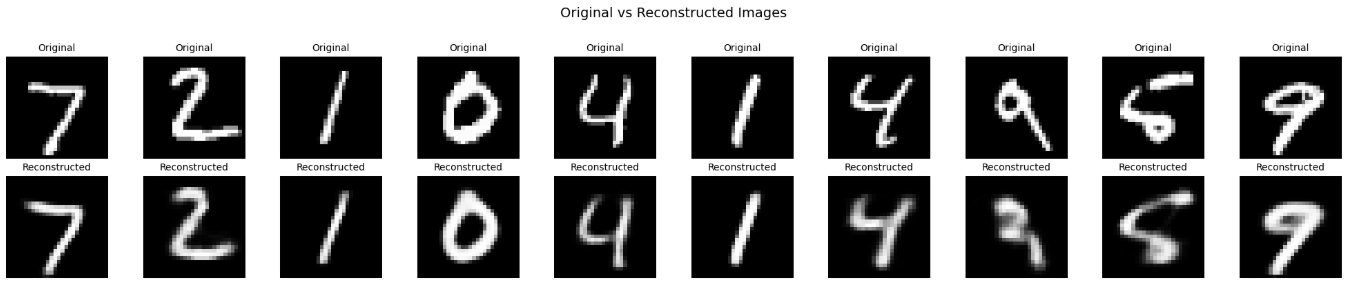
\includegraphics[width=1\textwidth]{image.png}
    \caption{Reconstructed images from the MNIST using the VAE.}
    \label{fig:image}
\end{figure}

\noindent The reconstructed images are expected to be slightly blurrier than the originals because the VAE decoder must synthesise outputs from a \emph{sampled} (not exact) latent code. This blurriness is a direct consequence of averaging over the posterior distribution — it is a known characteristic of VAEs and a trade-off for obtaining a smooth, continuous latent space that supports generation.

% -------------------------------------------------------
%  SECTION 6 -- DISCUSSION
% -------------------------------------------------------
\section{Discussion}

\subsection{Why the Reparameterization Trick Is Essential}

Without this trick, the gradient of the loss with respect to $\boldsymbol{\mu}$ and $\boldsymbol{\sigma}$ would need to pass through a stochastic node — an operation undefined for standard automatic differentiation. Score-function estimators (REINFORCE) exist as an alternative but have extremely high variance. The reparameterization trick provides a low-variance, unbiased gradient estimate at no additional computational cost, making VAE training practical and stable.

\subsection{Latent Space Continuity}

The KL divergence term penalises encoders that map inputs to overly narrow or displaced Gaussians. This forces the posterior $q_\phi(\mathbf{z}|\mathbf{x})$ to remain close to the prior $\mathcal{N}(\mathbf{0},\mathbf{I})$, resulting in a latent space where nearby points decode into semantically similar images. This is the property that enables smooth interpolation and controlled generation — both impossible in a standard autoencoder.

\subsection{VAE vs.\ Standard Autoencoder — Summary}

A standard autoencoder encodes $\mathbf{x}$ to a single point $\mathbf{z}$: expressive but unstructured. A VAE encodes $\mathbf{x}$ to a \emph{region} (a Gaussian) in latent space, balancing expressiveness against regularisation. The reparameterization trick is the bridge that allows this probabilistic formulation to be trained end-to-end with gradient descent, giving the VAE its generative power while retaining the reconstruction accuracy of the autoencoder.

% -------------------------------------------------------
%  SECTION 7 -- CONCLUSION
% -------------------------------------------------------
\section{Conclusion}

This report presented the complete design and implementation of a Variational Autoencoder for MNIST digit reconstruction. The reparameterization trick — implemented via \texttt{z = mu + exp(0.5 * log\_var) * eps}, where \texttt{eps $\sim$ N(0,I)} — is the cornerstone of the approach: it converts an intractable stochastic gradient problem into a straightforward deterministic one. The combined BCE + KLD loss function trains the model to simultaneously reconstruct inputs faithfully and maintain a well-structured Gaussian latent space. This architecture is fundamentally superior to a standard autoencoder for generative tasks, offering smooth latent interpolation, controllable sampling, and principled uncertainty estimation.

\end{document}